%auto-ignore
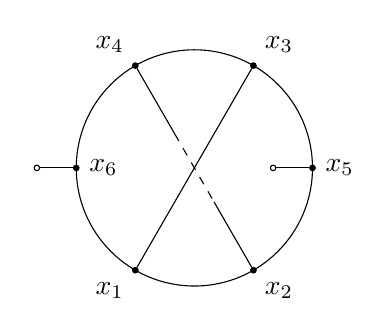
\begin{tikzpicture}
 \tikzset{point/.style = {draw, circle, fill=black, minimum size=2pt,inner sep=0pt}}
 \tikzset{->-/.style={decoration={markings,mark=at position #1 with {\arrow{>}}},postaction={decorate}}}
 
 \def\rad{1.5cm}
 \def\ang{60}
 \def\dashsep{0.5cm}
 \def\lenext{0.5cm}
 
 \coordinate (C) at (0,0);
 \draw (C) circle (\rad);

 \path (C) node[point,label={0:$x_5$}] (x5)  at +(0*\ang:\rad){};
 \path (C) node[point,label={\ang:$x_3$}] (x3)  at +(1*\ang:\rad){};
 \path (C) node[point,label={2*\ang:$x_4$}] (x4)  at +(2*\ang:\rad){};
 \path (C) node[point,label={0:$x_6$}] (x6)  at +(3*\ang:\rad){};
 \path (C) node[point,label={4*\ang:$x_1$}] (x1)  at +(4*\ang:\rad){};
 \path (C) node[point,label={5*\ang:$x_2$}] (x2)  at +(5*\ang:\rad){};
 
 \draw (x5) -- +(180:\lenext) node[point,style={fill=white},label={90:$\NVol$}] {};
 \draw (x6) -- +(180:\lenext) node[point,style={fill=white},label={90:$\NVol$}] {};
 \draw (x1) -- (x3);
 
 \path (C) coordinate (p1)  at +(2*\ang:\dashsep){};
 \path (C) coordinate (p2)  at +(-1*\ang:\dashsep){};
 
 \draw (x2) -- (p2);
 \draw (x4) -- (p1);
 \draw[dashed] (p1) -- (p2);
\end{tikzpicture}